\documentclass{article}
\usepackage[utf8]{inputenc}
\usepackage[english,russian]{babel} 
\renewcommand{\AA}{\ensuremath{\mathring{A}}}

\title{Лабораторная работа № 1.2\\
Исследование эффекта Комптона}
\author{Руденко Ирина, 494}
\date{13 марта 2017}

\usepackage{natbib}
\usepackage{graphicx}

\usepackage{amsthm}
\newtheorem{definition}{Опредление}
\theoremstyle{remark}
\newtheorem*{remark}{Замечание}
\begin{document}
\maketitle

\textbf{В работе используются:}   толстостенный контейнет с коллиматором с размещённым в нём $^{137}Cs$, графитовая мишень, сцинтиляционный счётчик(сцинтилятором служит NaI(Tl), фотокатод ФЭУ, ЭВМ


\textbf{Цель работы:}  изучить поведение величины комптоновского смещения.

\begin{figure}[htp]
    \centering
    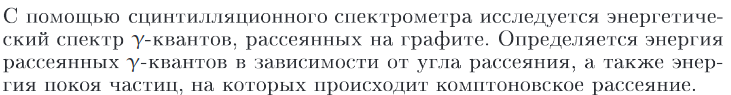
\includegraphics[width=1.1\linewidth]{1.png}

\end{figure}
\begin{figure}[htp]
    \centering
    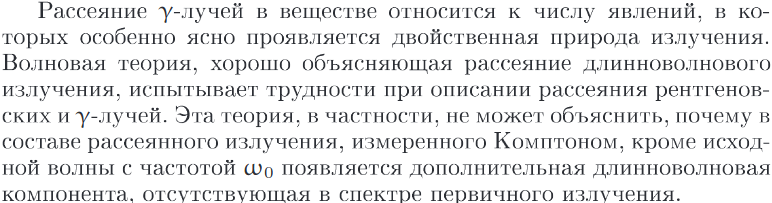
\includegraphics[width=1.2\linewidth]{2.png}
\end{figure}

\begin{figure}[htp]
    \centering
    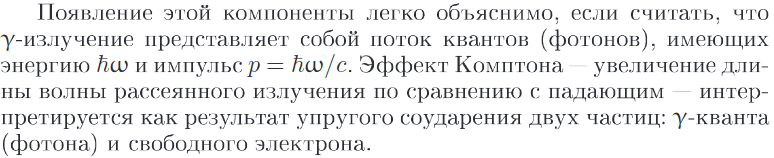
\includegraphics[width=1.2\linewidth]{3.png}
\end{figure}
\begin{figure}[htp]
    \centering
    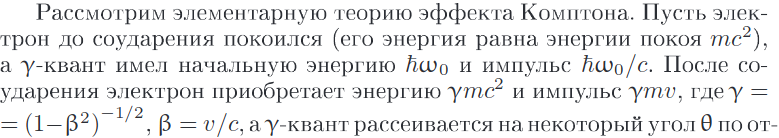
\includegraphics[width=1.2\linewidth]{4.png}
\end{figure}
\begin{figure}[htp]
    \centering
    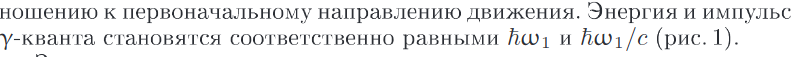
\includegraphics[width=1.2\linewidth]{5.png}
\end{figure}

\begin{figure}[htp]
    \centering
    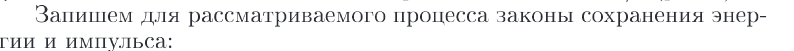
\includegraphics[width=1.2\linewidth]{6.png}
\end{figure}
\begin{figure}[htp]
    \centering
    
\includegraphics[width=1.2\linewidth]{7.png}
\end{figure}
\begin{figure}[htp]
    \centering
    
\includegraphics[width=1.2\linewidth]{8.png}
\end{figure}
\begin{figure}[htp]
    \centering
    
\includegraphics[width=1.2\linewidth]{9.png}
\end{figure}
\begin{figure}[htp]
    \centering
    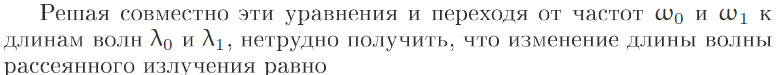
\includegraphics[width=1.2\linewidth]{10.png}
\end{figure}
\begin{figure}[htp]
    \centering
    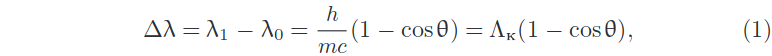
\includegraphics[width=1.2\linewidth]{11.png}
\end{figure}
\begin{figure}[htp]
    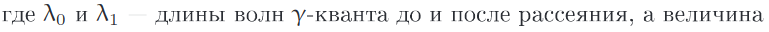
\includegraphics[width=1.2\linewidth]{12.png}
\end{figure}
\begin{figure}[htp]
    
\includegraphics[width=1.2\linewidth]{13.png}
\end{figure}
\begin{figure}[htp]
    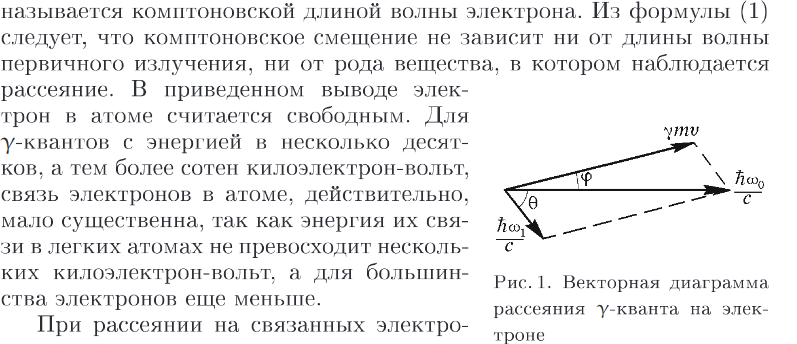
\includegraphics[width=1.2\linewidth]{14.png}
\end{figure}

\begin{figure}[htp]
    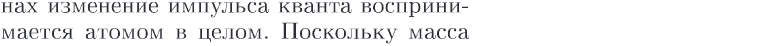
\includegraphics[width=1.2\linewidth]{15.png}
\end{figure}
\begin{figure}[htp]
    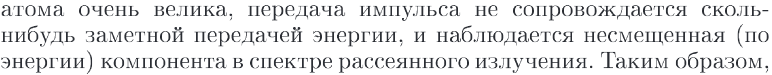
\includegraphics[width=1.2\linewidth]{16.png}
\end{figure}
\begin{figure}[htp]
    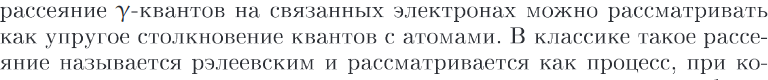
\includegraphics[width=1.2\linewidth]{17.png}
\end{figure}
\begin{figure}[htp]
    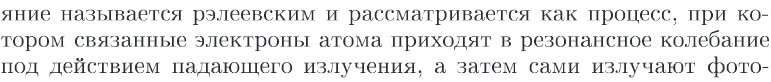
\includegraphics[width=1.2\linewidth]{18.png}
\end{figure}
\begin{figure}[htp]
    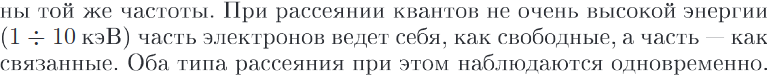
\includegraphics[width=1.2\linewidth]{19.png}
\end{figure}
\begin{figure}[htp]
    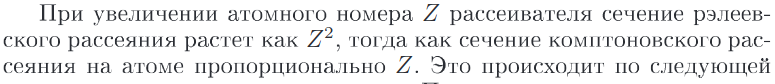
\includegraphics[width=1.2\linewidth]{20.png}
\end{figure}
\begin{figure}[htp]
    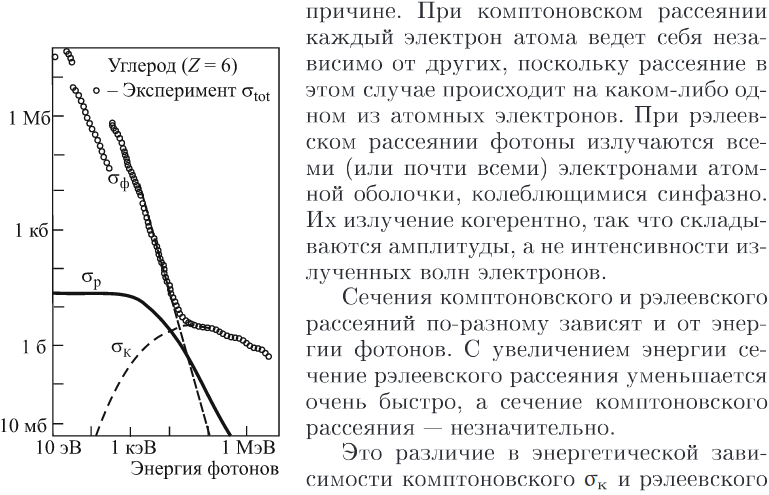
\includegraphics[width=1.2\linewidth]{21.png}
\end{figure}
\begin{figure}[htp]
    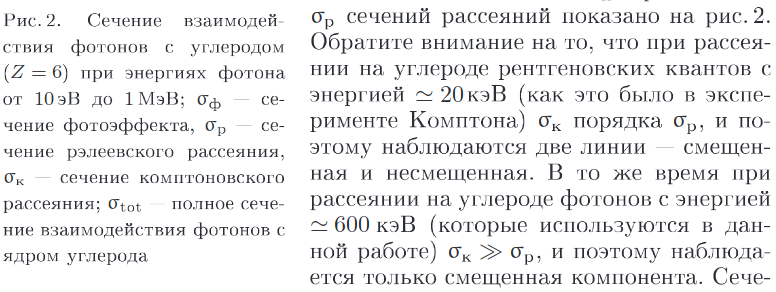
\includegraphics[width=1.2\linewidth]{22.png}
\end{figure}
\begin{figure}[htp]
    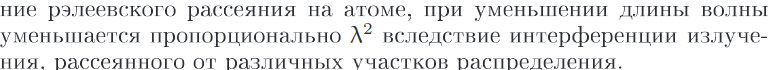
\includegraphics[width=1.2\linewidth]{23.png}
\end{figure}
\begin{figure}[htp]
    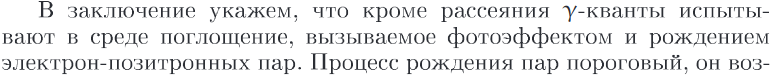
\includegraphics[width=1.2\linewidth]{24.png}
\end{figure}
\begin{figure}[htp]
    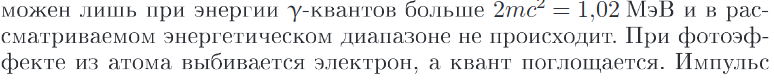
\includegraphics[width=1.2\linewidth]{25.png}
\end{figure}
\begin{figure}[htp]
    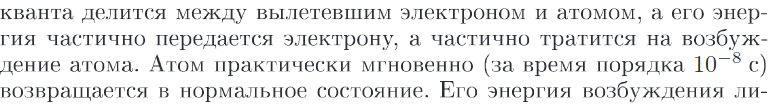
\includegraphics[width=1.2\linewidth]{26.png}
\end{figure}
\begin{figure}[htp]
    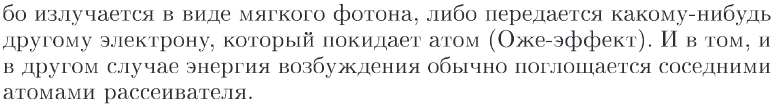
\includegraphics[width=1.2\linewidth]{27.png}
\end{figure}
\begin{figure}[htp]
    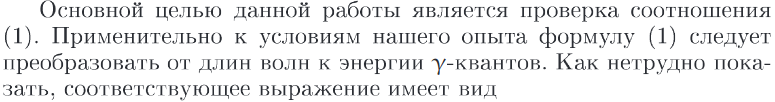
\includegraphics[width=1.2\linewidth]{28.png}
\end{figure}
\begin{figure}[htp]
    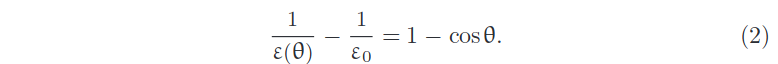
\includegraphics[width=1.2\linewidth]{29.png}
\end{figure}
\begin{figure}[htp]
    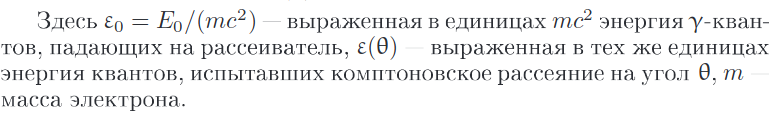
\includegraphics[width=1.2\linewidth]{30.png}
\end{figure}
\begin{figure}[htp]
    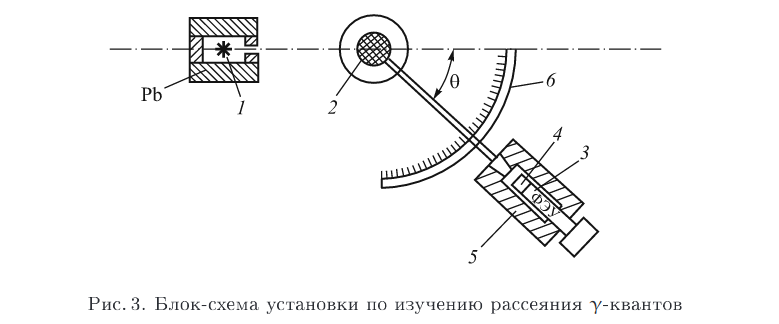
\includegraphics[width=1.2\linewidth]{31.png}
\end{figure}
\clearpage
\section{Ход работы:}

1. Постороим зависимость $\frac{1}{N(\theta)}$ от $1 - cos(\theta)$
\begin{figure}[htp]
    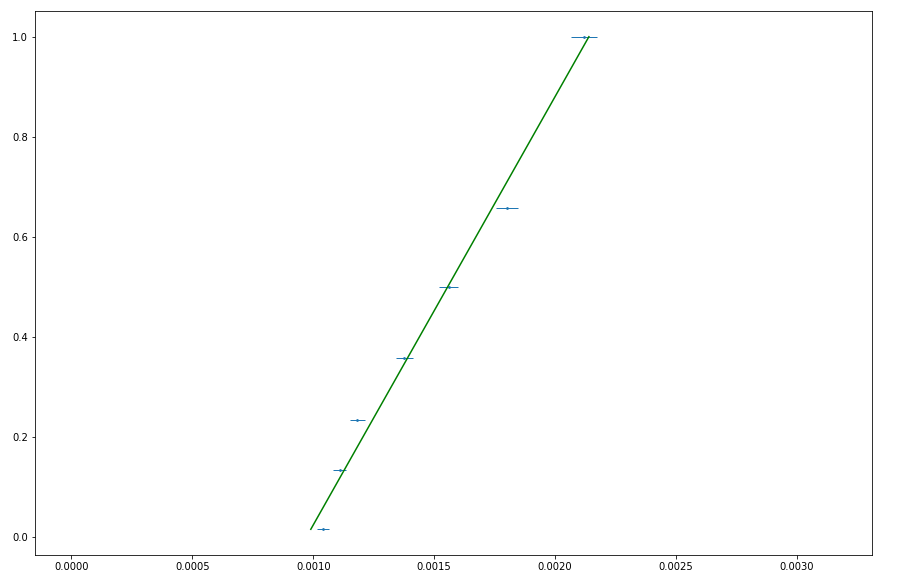
\includegraphics[width=1.2\linewidth]{36.png}
\end{figure}
2. Известно, что: $H_\gamma = 662 kEv$

$mc^2_{theory} = 511 kEv$

2. Полученные $N(0)_{best} = 1036\\$
$N(90)_{best} = 457$
$\sigma = 0.026$

\begin{equation}
    mc^2 = E_\gamma \cdot \frac{N(90)}{N(0) - N(90)} = 522.13 kEv
\end{equation}


3. Постороим общую зависимость для двух различных приборов  $\frac{1}{N(\theta)}$ от $1 - cos(\theta)$
\begin{figure}[htp]
    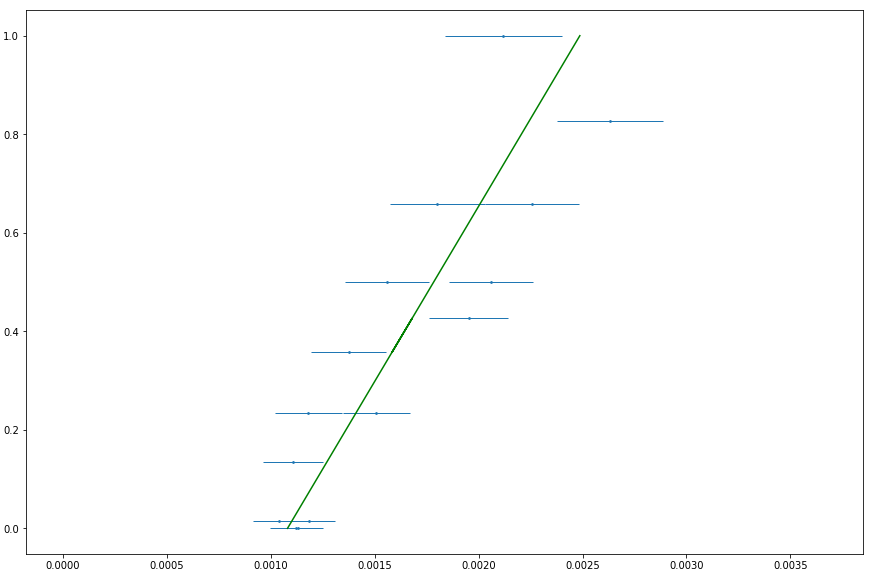
\includegraphics[width=1.2\linewidth]{35.png}
\end{figure}

4. Полученные $N(0)_{best} = 924\\$
$N(90)_{best} = 402$
$\sigma = 0.11$

\begin{equation}
    mc^2 = E_\gamma \cdot \frac{N(90)}{N(0) - N(90)} = 509  kEv
\end{equation}


\end{document}